\section{Resultados}

A continuación se presentan los resultados experimentales obtenidos durante los ensayos realizados en el laboratorio.

En el Cuadro~\ref{tab:parametros_config} se resumen los parámetros de configuración y dimensiones físicas de los equipos e instrumentos utilizados en la realización de las pruebas.

\begin{table}[H]
\centering
\caption{Parámetros de configuración del circuito experimental y dimensiones del núcleo}
\begin{tabularx}{\textwidth}{|X|Y|}
\hline
\textbf{Parámetro / Elemento} & \textbf{Valor / Dimensiones} \\ \hline
Capacitor ($C$) & $1\,\mu\text{F}$ \\ \hline
Resistencia de Shunt ($R_{\text{shunt}}$) & $10\text{ A} \rightarrow 50\text{ mV}$ \\ \hline
Sonda de corriente & $1\text{ mV} / 10\text{ mA}$ \\ \hline
Número de espiras ($N$) & Bobinas de $150$ vueltas \\ \hline
\end{tabularx}
\label{tab:parametros_config}
\end{table}

\begin{figure}[H]
\centering
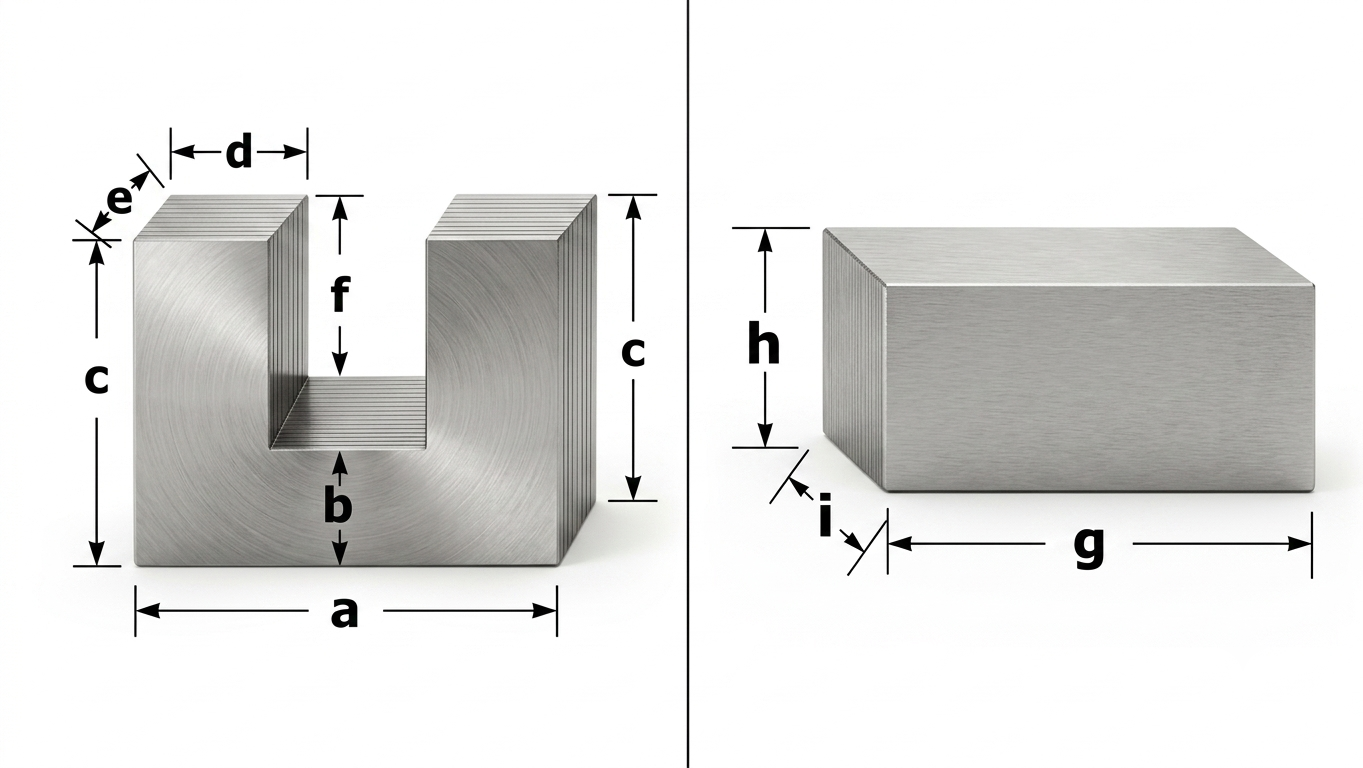
\includegraphics[width=0.75\textwidth]{imagenes/dimensiones-del-nucleo.png}
\caption{Dimensiones del núcleo utilizadas en el experimento.}
\label{fig:dimensiones_nucleo}
\end{figure}

\vspace{1em}

\subsection{Núcleo Macizo}

\begin{table}[H]
\centering
\caption{Dimensiones del núcleo macizo}
\begin{tabularx}{0.8\textwidth}{|X|X|}
\hline
 Constante  &   Dimensiones[cm] \\ \hline
     a      &       10,0 \\ \hline
     b      &       2,5 \\ \hline
     c      &       10,5 \\ \hline
     d      &       3,1 \\ \hline
     e      &       3,1 \\ \hline
     f      &       8,0  \\ \hline
     g      &       10,1 \\ \hline
     h      &       3,0 \\ \hline
     i      &       3,1 \\ \hline
\end{tabularx}
\label{Dimensiones del núcleo macizo}
\end{table}

\vspace{1em}

\begin{table}[H]
\centering
\caption{Mediciones experimentales para el ensayo de núcleo macizo (Ciclo de histéresis)}
\label{tab:nucleo_macizo}
\begin{tabularx}{\textwidth}{|Y|Y|Y|Y|}
\hline
\textbf{Voltaje nominal del VARIAC (V)} & \textbf{$V_{\text{RMS}}$ medido (V)} & \textbf{$I_{\text{RMS}}$ medida (A)} & \textbf{Potencia Activa $P$ (W)} \\ \hline
40 & $40 \pm 1$ & $3,8 \pm 0,1$ & $ 23 \pm 1$ \\ \hline
35 & $34 \pm 1$ & $3 \pm 0,1$ & $16 \pm 1$ \\ \hline
30 & $30 \pm 1$ & $2,5 \pm 0,1$ & $11 \pm 1$ \\ \hline
25 & $24 \pm 1$ & $1,9 \pm 0,1$ & $7 \pm 1$ \\ \hline
20 & $18 \pm 1$ & $1,3 \pm 0,1$ & $4 \pm 1$ \\ \hline
15 & $15 \pm 1$ & $1,1 \pm 0,5$ & $3 \pm 1$ \\ \hline
10 & $10 \pm 1$ & $0,8 \pm 0,1$ & $1 \pm 1$ \\ \hline
15 & $15 \pm 1$ & $1,1 \pm 0,1$ & $2 \pm 1$ \\ \hline
20 & $21 \pm 1$ & $1,6 \pm 0,5$ & $5 \pm 1$ \\ \hline
25 & $25 \pm 1$ & $2 \pm 0,1$ & $7 \pm 1$ \\ \hline
30 & $30 \pm 1$ & $2,5 \pm 0,1$ & $11 \pm 1$ \\ \hline
35 & $35 \pm 1$ & $3 \pm 0,1$ & $16 \pm 1$ \\ \hline
40 & $42 \pm 1$ & $3,9 \pm 0,1$ & $25 \pm 1$ \\ \hline
\end{tabularx}
\end{table}

A continuación se presenta el ciclo de histéresis visto en el osciloscopio para el núcleo macizo, así como las formas de onda del voltaje y la corriente.

\begin{figure}[H]
\centering
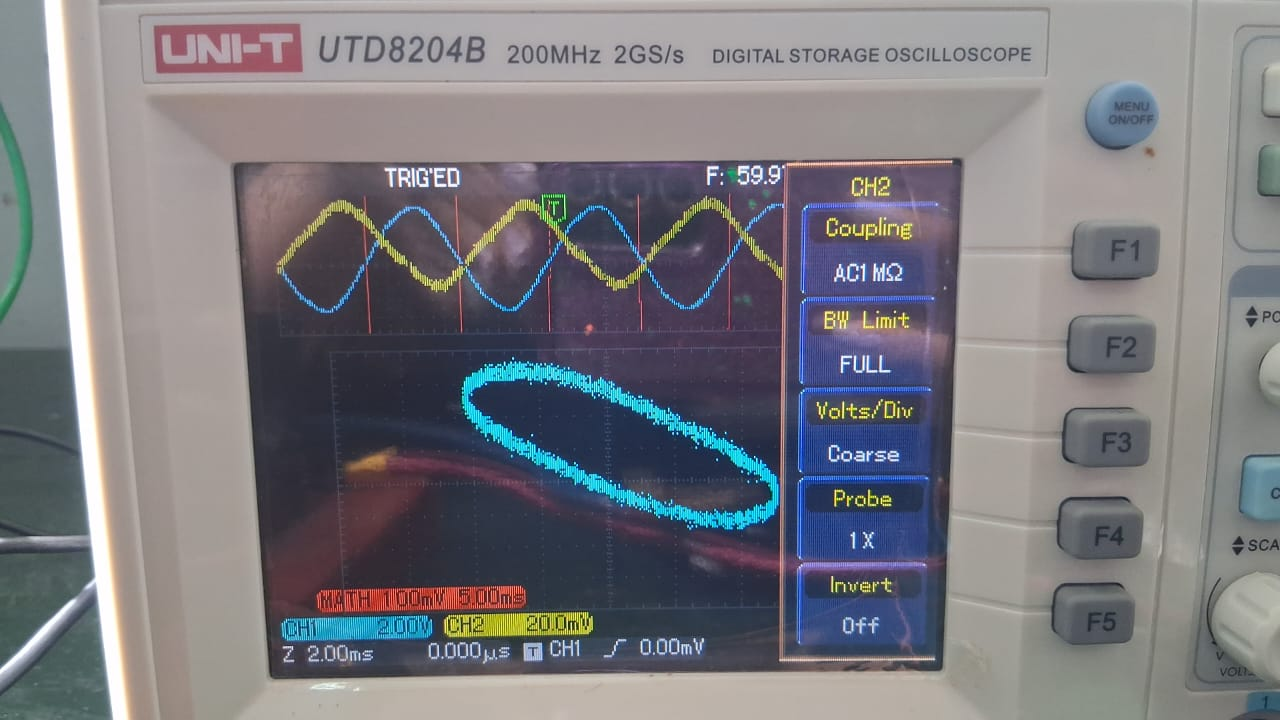
\includegraphics[width=0.7\textwidth]{imagenes/ciclo-histeresis-macizo.png}
\caption{Ciclo de histéresis obtenido experimentalmente para el núcleo macizo.}
\label{fig:ciclo_histeresis_macizo}
\end{figure}

\begin{figure}[H]
\centering
\begin{subfigure}[b]{0.48\textwidth}
    \centering
    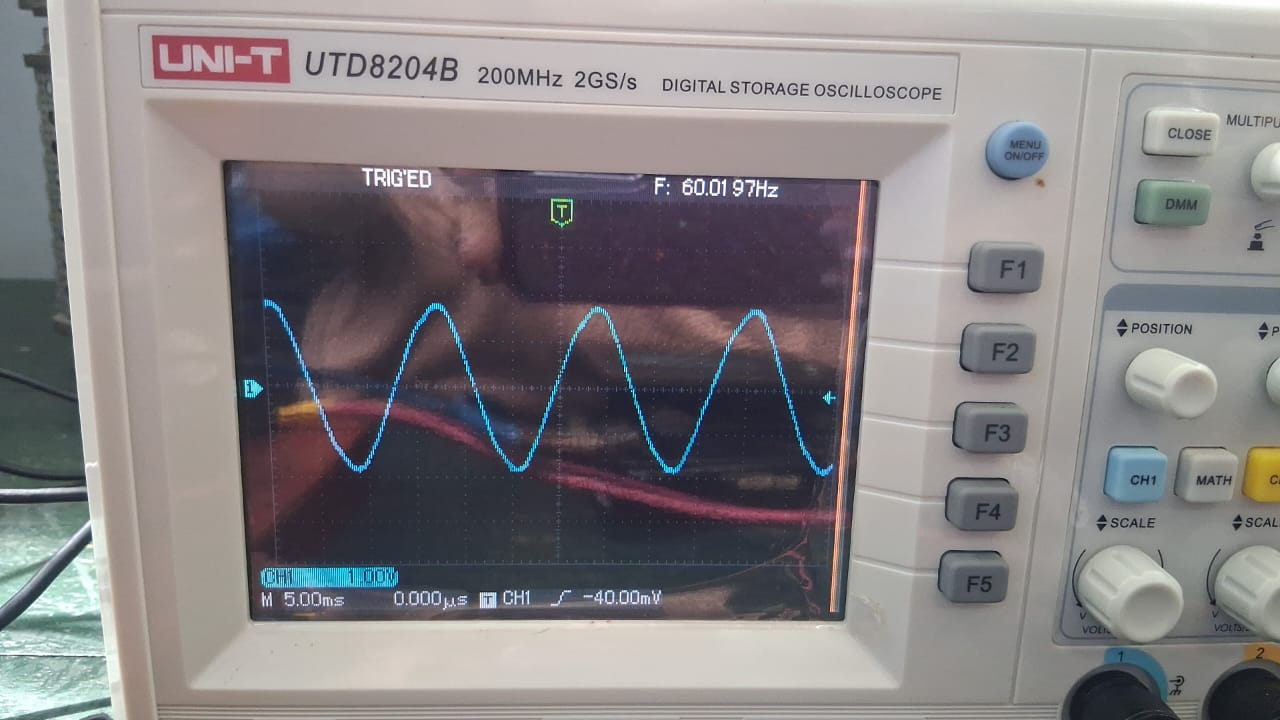
\includegraphics[width=\textwidth]{imagenes/onda-voltaje-nucleo-macizo.png}
    \caption{Forma de onda del voltaje.}
    \label{fig:onda_voltaje_macizo}
\end{subfigure}
\hfill
\begin{subfigure}[b]{0.48\textwidth}
    \centering
    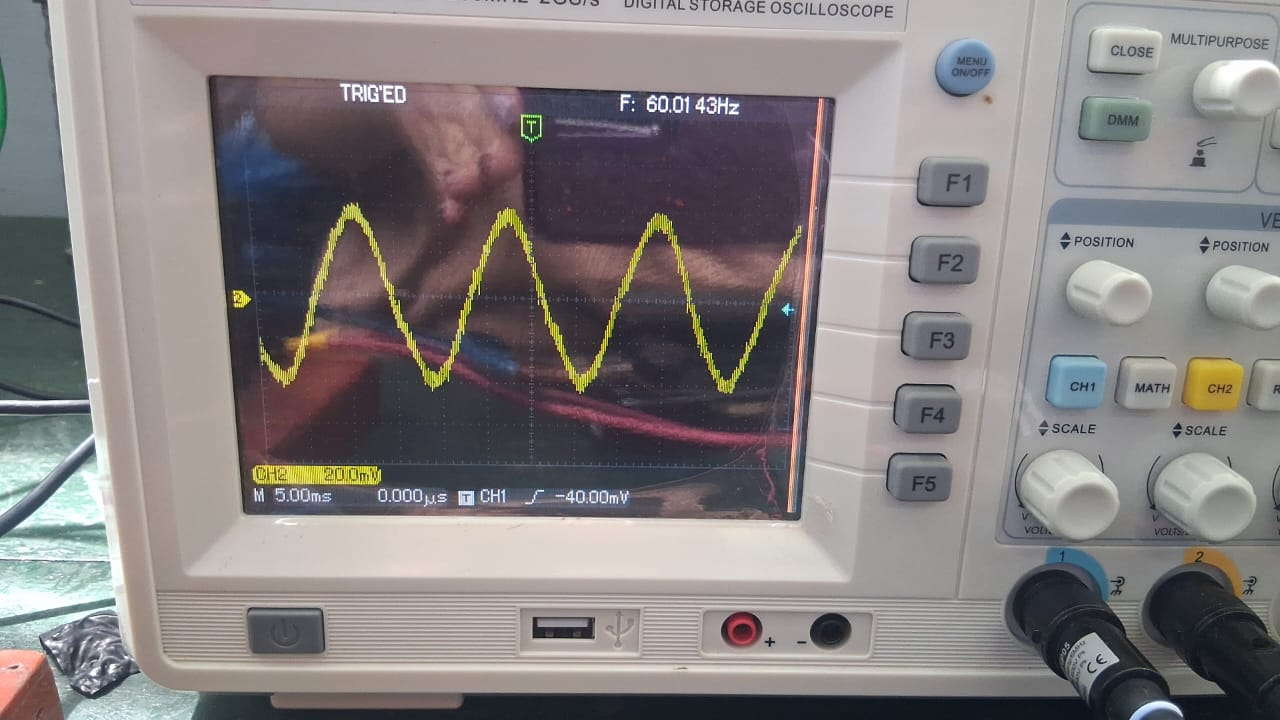
\includegraphics[width=\textwidth]{imagenes/onda-corriente-nucleo-macizo.png}
    \caption{Forma de onda de la corriente.}
    \label{fig:onda_corriente_macizo}
\end{subfigure}
\caption{Formas de onda en el núcleo macizo.}
\label{fig:formas_onda_macizo}
\end{figure}

\subsubsection{Cálculos correspondientes al núcleo macizo}
\begin{itemize}
    \item Determinar el factor de escala vertical $K_V$
        \begin{equation}
            K_V = \frac{V_{c}*C*R}{N_{2}*A}
        \end{equation}
    
    Se calculará el área de la sección transversal del núcleo y $R_s$
    \begin{equation}
        A = d \cdot e = 9,61 \text{ cm}^2  
    \end{equation}

    Para calcular la resistencia de shunt se usará las especificaciones del fabricante, que indican que para una corriente de 10A se obtiene una caída de tensión de 50mV. Por lo tanto, la resistencia de shunt se calcula como:

    \begin{equation}
        R_s = \frac{V}{I} = \frac{50 mV}{10A} = 5 m\Omega
    \end{equation}

    Los demás valores son conocidos: \newline
    $R = 150 k\Omega$                          \newline
    $V_c = 1,8\,\text{ mV}$           \newline
    $C = 1\,\mu\text{ F}$             \newline
    $N_2 = 150\ \text{ vueltas}$      \newline

    \begin{equation}
        K_V = \frac{(1,8\times 10^{-3}\,\text{V})(1\,\mu\text{F})(150k\Omega)}{(150\,\text{vueltas})(9,61\times 10^{-4}\,\text{m}^2)} = 1,87\times 10^{-3} [Tesla/div]
    \end{equation}
         
    \item Determinar el factor de escala horizontal $K_H$
        \begin{equation}
            K_H = \frac{N_1*V_s}{R_s*L}
        \end{equation}

    Se va a calcular la longitud media del camino magnético $L$ a partir de las dimensiones del núcleo macizo, utilizando la fórmula:
    \begin{equation}
        L = a - 2\frac{d}{2} + 2(c-\frac{b}{2}) + (g-\frac{d}{2}) = 33,93 \text{cm}= 0,3393 \text{m}
    \end{equation}

    Los demás valores son conocidos: \newline
    $N_1 = 300\ \text{ vueltas}$      \newline
    $V_s = 16\ \text{ mV}$            \newline
    $R_s = 5\ \text{ m}\Omega$         \newline
    $L = 0,3393\ \text{ m}$            \newline

    \begin{equation}
        K_H = \frac{(300 vueltas)( 16\times 10^{-3}\,\text{V})}{(5\times 10^{-3}\Omega)(0,3393\,\text{m})} = 2,829\,\text{k A/m/div}
    \end{equation}

    \item Determinar la energía
    
    Al observar la figura \ref{fig:ciclo_histeresis_macizo} se puede apreciar el ciclo de histéresis y a partir de las dimensiones y el área del ciclo se puede determinar la energía, en este caso:
    \begin{equation}
    W = 4 * K_V * K_H = 4 * 1,87 \times 10^{-3} * 2,829 k = 21,19 J
    \end{equation}

    \item Determinar la potencia disipada por histéresis
    \begin{equation}
        P_h= W * f * A * L
    \end{equation}

    Al sustiurir los valores conocidos, se obtiene:
    $$P_h = 0,39 \text{ W}$$

    \item Determinar la potencia en el núcleo
    \begin{equation}
        P_{núcleo} = P_h - P_f
    \end{equation}

    Conociendo que $P_{núcleo} = 23 W$ y $P_h = 0,39 W$, se puede determinar la potencia disipada por corrientes de Foucault

    \begin{equation}
        P_f = P_{núcleo} - P_h = 22,61 W
    \end{equation}
    
\end{itemize}
    
\vspace{1em}

\subsection{Núcleo laminado}

\begin{table}[H]
\centering
\caption{Dimensiones del núcleo laminado}
\begin{tabularx}{0.8\textwidth}{|X|X|}
\hline
 Constante  &   Dimensiones[cm] \\ \hline
     a      &       10,1 \\ \hline
     b      &       3,0  \\ \hline
     c      &       10,1 \\ \hline
     d      &       3,0 \\ \hline
     e      &       3,0 \\ \hline
     f      &       8,0  \\ \hline
     g      &       10,0 \\ \hline
     h      &       3,0 \\ \hline
     i      &       3,0 \\ \hline
\end{tabularx}
\label{Dimensiones del núcleo laminado}
\end{table}

\begin{table}[H]
\centering
\caption{Mediciones experimentales para el ensayo de núcleo laminado}
\label{tab:nucleo_laminado}
\begin{tabularx}{\textwidth}{|Y|Y|Y|Y|}
\hline
\textbf{Voltaje nominal del VARIAC (V)} & \textbf{$V_{\text{RMS}}$ medido (V)} & \textbf{$I_{\text{RMS}}$ medida (A)} & \textbf{Potencia Activa $P$ (W)} \\ \hline
110 & $110 \pm 1$ & $3 \pm 0,1$ & $10 \pm 1$ \\ \hline
100 & $100 \pm 1$ & $2 \pm 0,1$ & $6 \pm 1$ \\ \hline
80 & $80 \pm 1$ & $0,9 \pm 0,3$ & $4 \pm 1$ \\ \hline
60 & $60 \pm 1$ & $0,3 \pm 0,1$ & $2 \pm 1$ \\ \hline
40 & $40 \pm 1$ & $0,2 \pm 0,1$ & $1 \pm 1$ \\ \hline
50 & $50 \pm 1$ & $0,2 \pm 0,1$ & $2 \pm 1$ \\ \hline
60 & $65 \pm 1$ & $0,4 \pm 0,1$ & $3 \pm 1$ \\ \hline
80 & $80 \pm 1$ & $0,9 \pm 0,1$ & $4 \pm 1$ \\ \hline
100 & $100 \pm 1$ & $2 \pm 0,1$ & $7 \pm 1$ \\ \hline
120 & $100 \pm 1$ & $3 \pm 0,1$ & $10 \pm 1$ \\ \hline
\end{tabularx}
\end{table}

\vspace{2em}

A continuación se presenta el ciclo de histéresis visto en el osculoscopio para el núcleo laminado.

\begin{figure}[H]
\centering
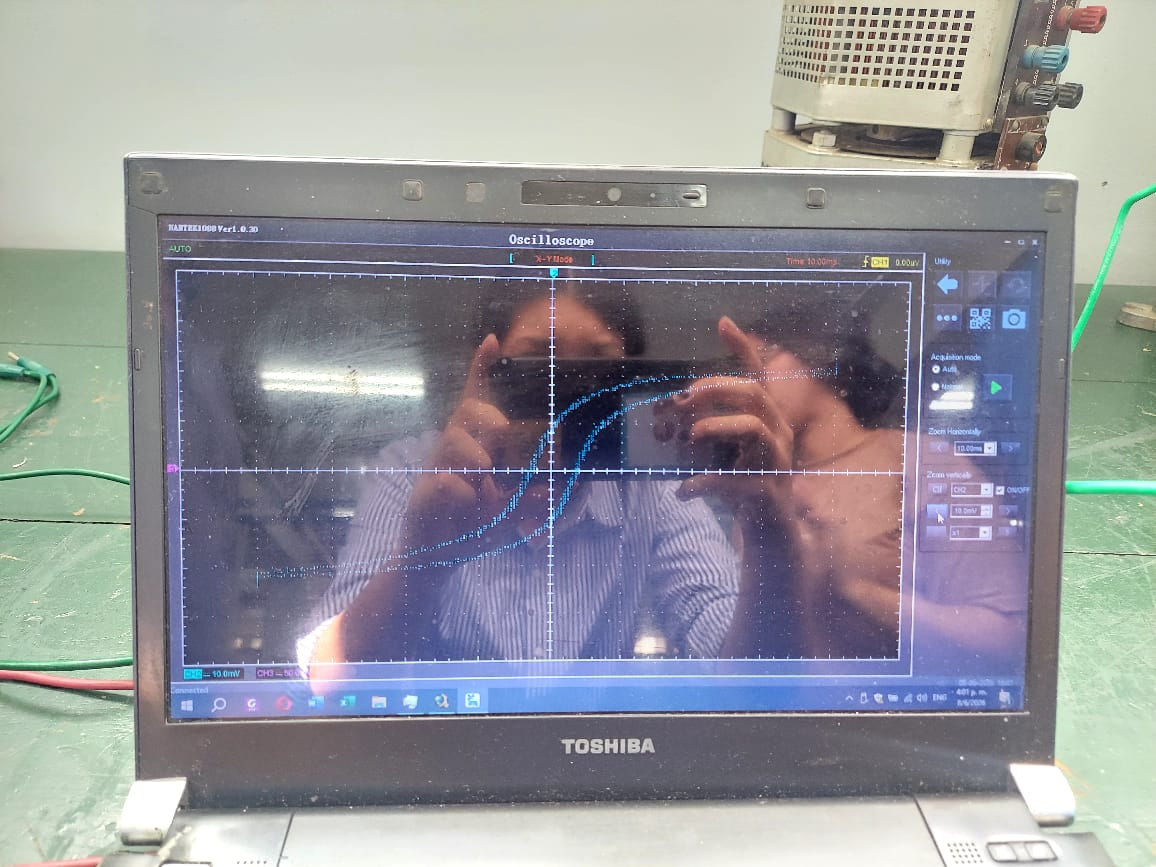
\includegraphics[width=0.7\textwidth]{imagenes/ciclo-histeresis-laminado.png}
\caption{Ciclo de histéresis obtenido experimentalmente para el núcleo laminado.}
\label{fig:ciclo_histeresis_laminado}
\end{figure}

\subsubsection{Cálculos correspondientes al núcleo laminado}
\begin{itemize}
    \item Determinar el factor de escala vertical $K_V$
        \begin{equation}
            K_V = \frac{V_{c}*C*R}{N_{2}*A}
        \end{equation}
    
    Se calculará el área de la sección transversal del núcleo y $R_s$
    \begin{equation}
        A = d \cdot e = 9,0 \text{ cm}^2  
    \end{equation}

    Los demás valores son conocidos: \newline
    $V_c = 10\,\text{mV}$                    \newline
    $C = 1\,\mu\text{F}$                  \newline
    $N_2 = 150\ \text{vueltas}$              \newline
    $R = 150 k\Omega$                          \newline

    \begin{equation}
            K_V = \frac{(10\,\text{mV})(1\,\mu\text{F})(150 \times 10^3\,\Omega)}{(150\,\text{vueltas})(9,0 \times 10^{-4}\,\text{m})} = 0,011 [Tesla/div]
    \end{equation}

    \item Determinar el factor de escala horizontal $K_H$
    
        \begin{equation}
            K_H = \frac{N_1*V_s}{R_s*L}
        \end{equation}

    Se va a calcular la longitud media del camino magnético $L$ a partir de las dimensiones del núcleo macizo, utilizando la fórmula:
    \begin{equation}
        L = a - 2\frac{d}{2} + 2(c-\frac{b}{2}) + (g-\frac{d}{2}) = 32,8 \text{cm}= 0,328 \text{m}
    \end{equation}

    Los demás valores son conocidos: \newline
    $N_1 = 300\ \text{ vueltas}$      \newline
    $V_s = 40\ \text{ mV}$            \newline
    $R_s = 5\ \text{ m}\Omega$         \newline
    $L = 0,328\ \text{ m}$            \newline

    \begin{equation}
        K_H = \frac{(300 vueltas)( 40 mV)}{(5 m\Omega)(0,328 m)} = 7,317 k A/m.div
    \end{equation}

    \item Determinar la energía
    
    Al observar la figura \ref{fig:ciclo_histeresis_laminado} se puede apreciar el ciclo de histéresis y a partir de las dimensiones y el área del ciclo se puede determinar la energía, en este caso:
    \begin{equation}
    W = 4 * K_V * K_H = 4 * 0,011 * 7,317 k = 325,20 J
    \end{equation}

    \item Determinar la potencia disipada por histéresis
    \begin{equation}
        P_h= W * f * A * L
    \end{equation}

    Al sustiurir los valores conocidos, se obtiene:
    $$P_h = 5.94 \text{ W}$$

    \item Determinar la potencia en el núcleo
    \begin{equation}
        P_{núcleo} = P_h - P_f
    \end{equation}

    Conociendo que $P_{núcleo} = 10 W$ y $P_h = 5.94 W$, se puede determinar la potencia disipada por corrientes de Foucault

    \begin{equation}
        P_f = P_{núcleo} - P_h = 4.24 W
    \end{equation}

\end{itemize}


